\chapter{Patient}
Ved implementering af en ny teknologi, herunder en Ultralyds Robotarm, kan det have en indvirkning på patienten. Derfor er det vigtig at belyse, hvilken effekt den nye teknologi har på patientgruppen. \\
I denne MTV vil både gravide og sonografer blive placeret i rollen som patienter. Gravide da de får foretaget en ultralydscanning og sonografer da de ofte oplever arbejdskader. Begge grupper vil derfor blive belyst i dette afsnit.  
\newline
For at kunne udarbejde en fyldestgørende analyse af patientperspektivet er det nødvendigt at belyse flere forhold. Se figur \ref{patientMTV}, hvor de fem patientperspektiver er vist. 
\begin{figure}[h!]\centering
	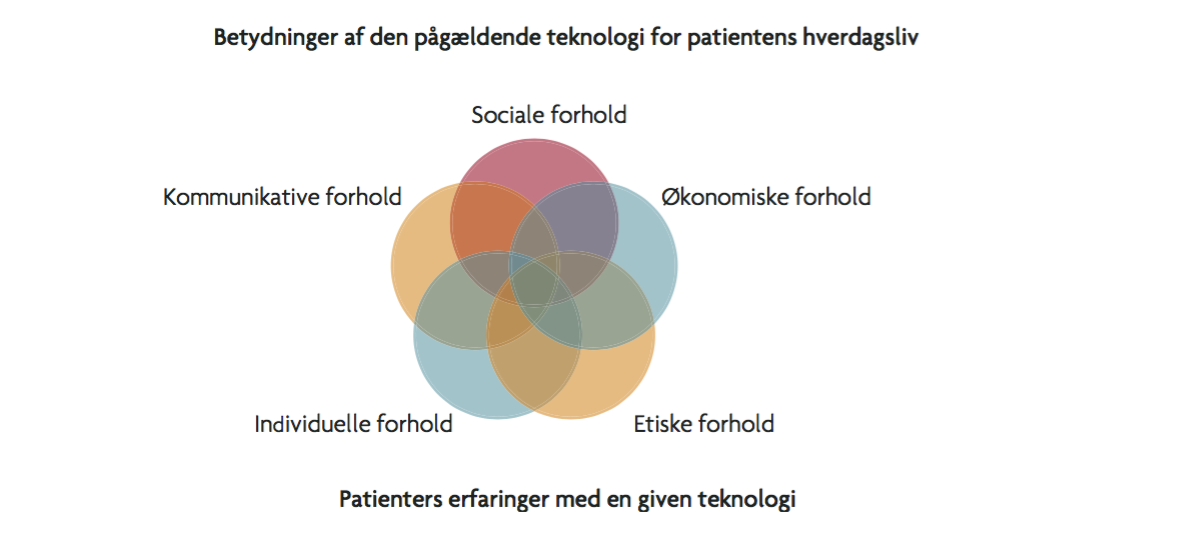
\includegraphics[width = 1.0\textwidth]{Figurer/PatientaspekterMTV}
	\caption{Udforskning af de fem patientaspekter i MTV, som har betydning for patientens hverdagsliv}
	\label{patientMTV}
\end{figure}

\section{Sociale forhold }
\section{Kommunikative forhold}

\section{Individuelle forhold}
\section{Etiske forhold}
Brugen af en Ultralyds Robotarm danner grundlag for en række etiske problemstillinger, som påvirker både gravide og personalet. 
Problemstillingerne omhandler de professionsetiske principper \cite{Husted}: 
\begin{itemize}
	\item \textbf{Pligter}
	\begin{itemize}
		\item Undgå skade af brugeren:\\ 
		Ultralyds Robotarmen skal hverken være til skade for gravide eller personalet. 
	\end{itemize} 
	\item \textbf{Konsekvenser}
	\begin{itemize}
		\item Forebygge sygdom og sygelighed og fremme sundhed eller status quo: \\
		Hvis man ud fra et nytteetisk perspektiv, kan få flere gravide igennem en scanning på kortere tid og samtidig mindske antallet af arbejdsskader for personalet, vil ressourcerne blive udnyttet bedst muligt, og derved komme flest mulige til gavn. Dette følger de socialetiske tanker, som tager hensyn til de mange.    
		\item Lindre lidelse, fremmedgørelse og ubehag:\\
		Ultralyds Robotarmen skal opfylde dette overfor personalet og patienten. Patienten kan føle sig fremstillet som et objekt,  da teknologien kommer tættere på patienten, mens personalet kommer længere væk. Dog er personale til stede i samme rum som patienten, derved er der stadig en form for menneskelig kontakt.  
	\end{itemize}
	\item \textbf{Idealer}
	\begin{itemize}
		\item Handle med forståelse og empati:\\
		Der sker en ændring af nærhed- og omsorgsrelationen mellem den gravide og personalet under en scanning med Ultralyds Robotarmen. 
		\item Handle med etik ansvarlighed overfor personalet:\\
		Ultralyds Robotarmen skal være ansvarlig over for personalet idet at der skal være empati for arbejdssituationen.\\
		Resultatet er at en mindskelse i antallet af arbejdsskader, fremmer personalesikkerhed og -trivsel.   		
	\end{itemize} 
\end{itemize} 

\section{Økonomiske forhold}

\section{Delkonklusion }